\begin{figure*}
  \centering
  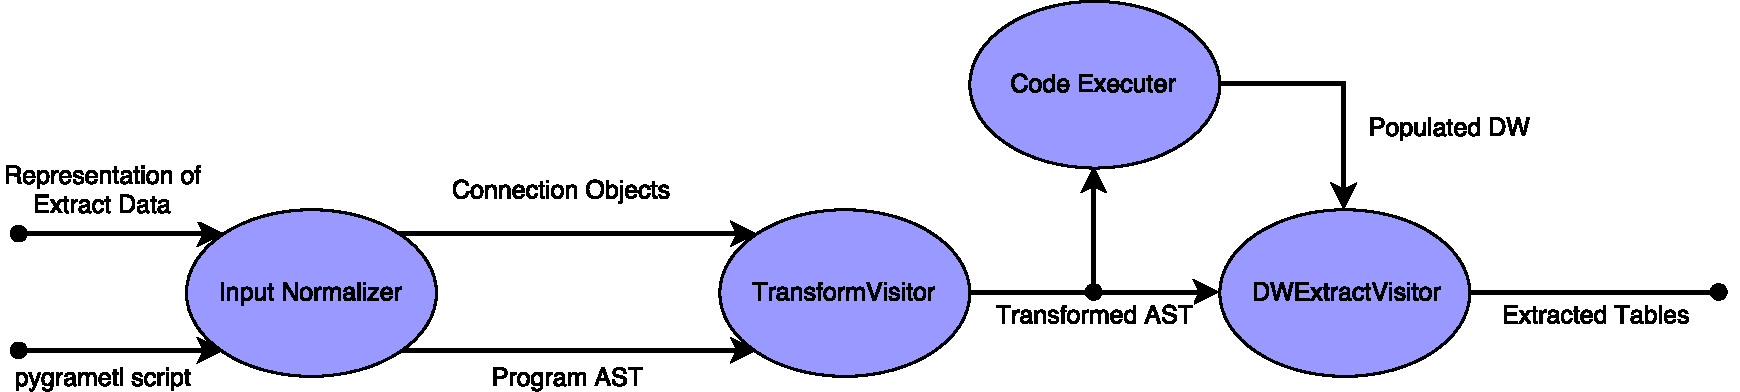
\includegraphics[width=1\textwidth]{figures/reinterpreter_model.pdf}
  \label{fig:reinterpreter}
  \caption{Model of our Reinterpreter}
\end{figure*}

\section{pygrametl Reinterpreter}
For the sake of usability, we would like users to be able to give an arbitrary pygrametl program and a set of input data to \FW. \FW~should then be able to transform and execute the given pygrametl program in such a way that we use the given input data. We then need to be able to extract the data from the resulting populated data warehouse. These requirements can be divided into the following four individual subproblems.

\begin{itemize}
\item How should users specify their inputs and how do we normalize it?
\item How do we transform the pygrametl program to use these input?
\item How do we execute the transformed pygrametl program?
\item How do we represent the resulting data warehouse for our predicates and how do we extract it?
\end{itemize}

To solve these subproblems we have come up with a model for a reinterpreter seen in \cref{fig:reinterpreter}. This model describes how data will flow from object to object, where each object represents a solutions to each of the subproblems. This reinterpreter would be able to take any dataform supported by the \textit{InputNormalizer} as input data for the pygrametl program. It would then make the required changes to the pygrametl program by parsing the program and making changes to its AST using the \textit{TransformVisitor}. The resulting transformed AST can then be executed by the \textit{CodeExecuter}, which results in a data warehouse being populated. Lastly the \textit{DWExtractVisitor} will be able to extract the different tables from the populated data warehouse, by using retrieving schema information from the transformed AST.

The rest of this section will go further into depth with how these four objects are implemented.

\subsection{InputNormalizer}
\todo[inline]{NOT YET IMPLEMENTED: THIS IS SOME DRAFT STUFF}
The \textit{InputNormalizer} has three main functionalities, it has to parse the pygrametl program, it has to supply variable names to the \textit{TransformVisitor}, and it has to build a scope for the \textit{CodeExecuter}.

Parsing the pygrametl program is done using the default python package, \texttt{ast}. This however limits us to only reinterpreting pygrametl scripts that contains all the necessary information required for later use.

We would like to support as many representations of extract data for the ETL process as possible. And as such, bla blah blaah. \todo[inline]{Når vi engang har implementeret InputNormalizeren, så skriv lidt om hvordan den fungere her. Det tænkes at den bliver modulær og nok bruger noget dependency injection. Sådan at man nemt kan tilføje flere måder at give Extract Data på}


\subsection{TransformVisitor}
The \textit{TransformVisitor} has two main functionalities, for one, it must make certain that the user  given data is used instead of what is usually used by a pygrametl program. Secondly, it should also make sure that no connection objects are closed prematurely. 

For the first functionality, it will use the given AST of the pygrametl program to find instantiations of pygrametl datasource objects. For these it will replace either the connection parameter, for SQL type datasource objects, or the filename paramter, for CSV type datasource objects, with a variable name that was set by the \textit{InputNormalizer} and maps to a connection/filename. This way, whenever these sources are used in the future, they will connect to and use the user specified data.

For the second functionality, we simply make sure that if we assign a ConnectionWrapper to a variable, to make sure that the \texttt{close()} method is not called on this variable later on. And if it is, we delete the statement from the AST. This is done as we need to use the ConnectionWrappers connection later in the \textit{DWExtractVisitor} when we wish to access the populated data warehouse again.

\subsection{CodeExecuter}
The \textit{CodeExecuter}s only function is to execute the transformed AST it recieves from the \textit{TransformVisitor}. It does this by compiling the AST using the build-in python function \texttt{compile()}, and then executing the compilation using the build-in function \texttt{exec()}. Note, that when executing the compilation, we have to do so in a scope where the variable names we exchanged with the connections/filenames in the \textit{TransformVisitor}, map to the actual values we want. This is done by giving a dictionary that does just that, as the \texttt{locals} parameter to the \texttt{exec()} function.

Executing the transformed pygrametl program should then have the desired side effect of populating the data warehouse, using the user specified input data.

\subsection{DWExtractVisitor}
The \textit{DWExtractVisitor}s only function is to build a \textit{DWReprensentation} object, that can later be used by predicates.

The \textit{DWExtractVisitor} works by taking the connection used by the ConnectionWrapper, and uses this as a connection to the data warehouse. It then builds a \textit{DimRepresentation} and \textit{FTRepresentation} for each Dimension and FactTable instantiation in the pygrametl program. It gathers information about table name and attributes from said instantiations. This does limit our users to only be able to instantiate their Dimensions and FactTables using hardcoded string values. As we cant extract the value of a variable through an AST. \todo[inline]{Vi har allerede kørt programmet på det her tidspunkt, kan vi ikke bare gemme Dims og FTs og så hente de værdier ud der. I stedet for at bruge AST'en. Dette gør at vi ikke har denne limitation.}

Once the \textit{DimRepresentation}s and \textit{FTRepresentation}s have been made, they are concatenated into the collection class \textit{DWRepresentation}. This can then later be used by the predicates.

\subsubsection{DWRepresentation}
\todo[inline]{Skrive lidt om hvorfor vi laver DWRep og hvad den indeholder}
